\ifx\wholebook\relax\else

% --------------------------------------------
% Lulu:

    \documentclass[a4paper,12pt,twoside]{../includes/ThesisStyle}

	\usepackage[T1]{fontenc} %%%key to get copy and paste for the code!
%\usepackage[utf8]{inputenc} %%% to support copy and paste with accents for frnehc stuff
\usepackage{times}
\usepackage{ifthen}
\usepackage{xspace}
\usepackage{alltt}
\usepackage{latexsym}
\usepackage{url}            
\usepackage{amssymb}
\usepackage{amsfonts}
\usepackage{amsmath}
\usepackage{stmaryrd}
\usepackage{enumerate}
\usepackage{cite}
%\usepackage[pdftex,colorlinks=true,pdfstartview=FitV,linkcolor=blue,citecolor=blue,urlcolor=blue]{hyperref}
\usepackage{xspace}
%\usepackage{graphicx}
\usepackage{subfigure}
\usepackage[scaled=0.85]{helvet}
        
        
\newcommand{\sepe}{\mbox{>>}}
\newcommand{\pack}[1]{\emph{#1}}
\newcommand{\ozo}{\textsc{oZone}\xspace}
\newcommand\currentissues{\par\smallskip\textbf{Current Issues -- }}

\newboolean{showcomments}
\setboolean{showcomments}{true}
\ifthenelse{\boolean{showcomments}}
  {\newcommand{\bnote}[2]{
	\fbox{\bfseries\sffamily\scriptsize#1}
    {\sf\small$\blacktriangleright$\textit{#2}$\blacktriangleleft$}
    % \marginpar{\fbox{\bfseries\sffamily#1}}
   }
   \newcommand{\cvsversion}{\emph{\scriptsize$-$Id: macros.tex,v 1.1.1.1 2007/02/28 13:43:36 bergel Exp $-$}}
  }
  {\newcommand{\bnote}[2]{}
   \newcommand{\cvsversion}{}
  } 


\newcommand{\here}{\bnote{***}{CONTINUE HERE}}
\newcommand{\nb}[1]{\bnote{NB}{#1}}
\newcommand{\fix}[1]{\bnote{FIX}{#1}}
%%%% add your own macros 

\newcommand{\sd}[1]{\bnote{Stef}{#1}}
\newcommand{\ja}[1]{\bnote{Jannik}{#1}}
\newcommand{\na}[1]{\bnote{Nico}{#1}}
%%% 


\newcommand{\figref}[1]{Figure~\ref{fig:#1}}
\newcommand{\figlabel}[1]{\label{fig:#1}}
\newcommand{\tabref}[1]{Table~\ref{tab:#1}}
\newcommand{\layout}[1]{#1}
\newcommand{\commented}[1]{}
\newcommand{\secref}[1]{Section \ref{sec:#1}}
\newcommand{\seclabel}[1]{\label{sec:#1}}

%\newcommand{\ct}[1]{\textsf{#1}}
\newcommand{\stCode}[1]{\textsf{#1}}
\newcommand{\stMethod}[1]{\textsf{#1}}
\newcommand{\sep}{\texttt{>>}\xspace}
\newcommand{\stAssoc}{\texttt{->}\xspace}

\newcommand{\stBar}{$\mid$}
\newcommand{\stSelector}{$\gg$}
\newcommand{\ret}{\^{}}
\newcommand{\msup}{$>$}
%\newcommand{\ret}{$\uparrow$\xspace}

\newcommand{\myparagraph}[1]{\noindent\textbf{#1.}}
\newcommand{\eg}{\emph{e.g.,}\xspace}
\newcommand{\ie}{\emph{i.e.,}\xspace}
\newcommand{\ct}[1]{{\textsf{#1}}\xspace}


\newenvironment{code}
    {\begin{alltt}\sffamily}
    {\end{alltt}\normalsize}

\newcommand{\defaultScale}{0.55}
\newcommand{\pic}[3]{
   \begin{figure}[h]
   \begin{center}
   \includegraphics[scale=\defaultScale]{#1}
   \caption{#2}
   \label{#3}
   \end{center}
   \end{figure}
}

\newcommand{\twocolumnpic}[3]{
   \begin{figure*}[!ht]
   \begin{center}
   \includegraphics[scale=\defaultScale]{#1}
   \caption{#2}
   \label{#3}
   \end{center}
   \end{figure*}}

\newcommand{\infe}{$<$}
\newcommand{\supe}{$\rightarrow$\xspace}
\newcommand{\di}{$\gg$\xspace}
\newcommand{\adhoc}{\textit{ad-hoc}\xspace}

\usepackage{url}            
\makeatletter
\def\url@leostyle{%
  \@ifundefined{selectfont}{\def\UrlFont{\sf}}{\def\UrlFont{\small\sffamily}}}
\makeatother
% Now actually use the newly defined style.
\urlstyle{leo}



	\usepackage{amsmath,amssymb}             % AMS Math
% \usepackage[french]{babel}
\usepackage[latin1]{inputenc}
\usepackage[T1]{fontenc}
\usepackage[left=1.5in,right=1.3in,top=1.1in,bottom=1.1in,includefoot,includehead,headheight=13.6pt]{geometry}
\renewcommand{\baselinestretch}{1.05}

\usepackage{multicol}

% Table of contents for each chapter

\usepackage[nottoc, notlof, notlot]{tocbibind}
\usepackage{minitoc}
\setcounter{minitocdepth}{1}
\mtcindent=15pt
% Use \minitoc where to put a table of contents

\usepackage{enumitem}

\usepackage{aecompl}

% Glossary / list of abbreviations

%\usepackage[intoc]{nomencl}
%\renewcommand{\nomname}{List of Abbreviations}
%
%\makenomenclature

% My pdf code

\usepackage[pdftex]{graphicx}
\usepackage[a4paper,pagebackref,hyperindex=true]{hyperref}

\usepackage{pgfplotstable,booktabs,colortbl}
\pgfplotsset{compat=1.8}

% Links in pdf
\usepackage{color}
\definecolor{linkcol}{rgb}{0,0,0.4} 
\definecolor{citecol}{rgb}{0.5,0,0} 

% Change this to change the informations included in the pdf file

% See hyperref documentation for information on those parameters

\hypersetup
{
bookmarksopen=true,
pdftitle="Sista: a Metacircular Architecture for Runtime Optimisation Persistence",
pdfauthor="Clement BERA", 
pdfsubject="Thesis", %subject of the document
%pdftoolbar=false, % toolbar hidden
pdfmenubar=true, %menubar shown
pdfhighlight=/O, %effect of clicking on a link
colorlinks=true, %couleurs sur les liens hypertextes
pdfpagemode=None, %aucun mode de page
pdfpagelayout=SinglePage, %ouverture en simple page
pdffitwindow=true, %pages ouvertes entierement dans toute la fenetre
linkcolor=linkcol, %couleur des liens hypertextes internes
citecolor=citecol, %couleur des liens pour les citations
urlcolor=linkcol %couleur des liens pour les url
}

% definitions.
% -------------------

\setcounter{secnumdepth}{3}
\setcounter{tocdepth}{1}

% Some useful commands and shortcut for maths:  partial derivative and stuff

\newcommand{\pd}[2]{\frac{\partial #1}{\partial #2}}
\def\abs{\operatorname{abs}}
\def\argmax{\operatornamewithlimits{arg\,max}}
\def\argmin{\operatornamewithlimits{arg\,min}}
\def\diag{\operatorname{Diag}}
\newcommand{\eqRef}[1]{(\ref{#1})}

\usepackage{rotating}                    % Sideways of figures & tables
%\usepackage{bibunits}
%\usepackage[sectionbib]{chapterbib}          % Cross-reference package (Natural BiB)
%\usepackage{natbib}                  % Put References at the end of each chapter
                                         % Do not put 'sectionbib' option here.
                                         % Sectionbib option in 'natbib' will do.
\usepackage{fancyhdr}                    % Fancy Header and Footer

% \usepackage{txfonts}                     % Public Times New Roman text & math font
  
%%% Fancy Header %%%%%%%%%%%%%%%%%%%%%%%%%%%%%%%%%%%%%%%%%%%%%%%%%%%%%%%%%%%%%%%%%%
% Fancy Header Style Options

\pagestyle{fancy}                       % Sets fancy header and footer
\fancyfoot{}                            % Delete current footer settings

%\renewcommand{\chaptermark}[1]{         % Lower Case Chapter marker style
%  \markboth{\chaptername\ \thechapter.\ #1}}{}} %

%\renewcommand{\sectionmark}[1]{         % Lower case Section marker style
%  \markright{\thesection.\ #1}}         %

\fancyhead[LE,RO]{\bfseries\thepage}    % Page number (boldface) in left on even
% pages and right on odd pages
\fancyhead[RE]{\bfseries\nouppercase{\leftmark}}      % Chapter in the right on even pages
\fancyhead[LO]{\bfseries\nouppercase{\rightmark}}     % Section in the left on odd pages

\let\headruleORIG\headrule
\renewcommand{\headrule}{\color{black} \headruleORIG}
\renewcommand{\headrulewidth}{1.0pt}
\usepackage{colortbl}
\arrayrulecolor{black}

\fancypagestyle{plain}{
  \fancyhead{}
  \fancyfoot{}
  \renewcommand{\headrulewidth}{0pt}
}

\usepackage{algorithm}
\usepackage[noend]{algorithmic}

%%% Clear Header %%%%%%%%%%%%%%%%%%%%%%%%%%%%%%%%%%%%%%%%%%%%%%%%%%%%%%%%%%%%%%%%%%
% Clear Header Style on the Last Empty Odd pages
\makeatletter

\def\cleardoublepage{\clearpage\if@twoside \ifodd\c@page\else%
  \hbox{}%
  \thispagestyle{empty}%              % Empty header styles
  \newpage%
  \if@twocolumn\hbox{}\newpage\fi\fi\fi}

\makeatother
 
%%%%%%%%%%%%%%%%%%%%%%%%%%%%%%%%%%%%%%%%%%%%%%%%%%%%%%%%%%%%%%%%%%%%%%%%%%%%%%% 
% Prints your review date and 'Draft Version' (From Josullvn, CS, CMU)
\newcommand{\reviewtimetoday}[2]{\special{!userdict begin
    /bop-hook{gsave 20 710 translate 45 rotate 0.8 setgray
      /Times-Roman findfont 12 scalefont setfont 0 0   moveto (#1) show
      0 -12 moveto (#2) show grestore}def end}}
% You can turn on or off this option.
% \reviewtimetoday{\today}{Draft Version}
%%%%%%%%%%%%%%%%%%%%%%%%%%%%%%%%%%%%%%%%%%%%%%%%%%%%%%%%%%%%%%%%%%%%%%%%%%%%%%% 

\newenvironment{maxime}[1]
{
\vspace*{0cm}
\hfill
\begin{minipage}{0.5\textwidth}%
%\rule[0.5ex]{\textwidth}{0.1mm}\\%
\hrulefill $\:$ {\bf #1}\\
%\vspace*{-0.25cm}
\it 
}%
{%

\hrulefill
\vspace*{0.5cm}%
\end{minipage}
}

\let\minitocORIG\minitoc
\renewcommand{\minitoc}{\minitocORIG \vspace{1.5em}}

\usepackage{multirow}
\usepackage{slashbox}

\newenvironment{bulletList}%
{ \begin{list}%
	{$\bullet$}%
	{\setlength{\labelwidth}{25pt}%
	 \setlength{\leftmargin}{30pt}%
	 \setlength{\itemsep}{\parsep}}}%
{ \end{list} }

\newtheorem{definition}{D�finition}
\renewcommand{\epsilon}{\varepsilon}

% centered page environment

\newenvironment{vcenterpage}
{\newpage\vspace*{\fill}\thispagestyle{empty}\renewcommand{\headrulewidth}{0pt}}
{\vspace*{\fill}}



	\graphicspath{{.}{../figures/}}
	\begin{document}
\fi

\chapter{Optimising Just-in-time compiler architectures}
\label{chap:stateOfTheArt}
\minitoc

The thesis focuses on the design and the implementation of an optimising JIT architecture for Pharo. The main goals of this architecture are to write the optimising JIT in Pharo itself and to have it running in the same runtime than the optimised application on top of the existing VM. The following few paragraphs introduce briefly the need of an optimising JIT for performance and how an optimising JIT improve performance of run programs. Concrete examples and references are present in the context of the two most popular optimising JIT architecture in Section \ref{sec:existing1} and \ref{sec:existing2}, which we call respectevily the function-based architecture and the metatracing architecture.

Standard object-oriented languages feature dynamic dispatch. This feature is typically present in the form of virtual calls: the function to activate for each virtual call depends on information available at runtime but not at compile-time. Because of dynamic dispatch, it is difficult for an ahead-of-time compiler to optimise efficiently the code to execute. This problem is especially important for languages where virtual calls are very common. In our case, in Pharo, every call is a virtual call.

To efficiently optimise code in a language featuring dynamic dispatch, one solution is to use an optimising JIT. A VM featuring an optimising JIT executes a given code snippet through different phases. The first runs of the code snippet are done through a slow execution path, such as an interpreter, which collects information about the running program while executing it. Once the code snippet has been run a significant number of times, the optimising JIT recompiles the code snippet at runtime to optimised native code. The compiler optimisations are directed by the runtime information collected during the first runs. Further uses of the same code snippet can be executed using the optimised version. The same code snippet can therefore be executed differently depending on how frequently it is run and how many times it has been executed since the last start-up. We call each different way the VM can execute the same code snippet a different \emph{tier}.

\paragraph{Multiple tiers.} As an optimising JIT requires runtime information to direct the compiler optimisations, high-performance VMs are implemented with at least two tiers. One tier, slow to execute code, is used for the first runs of a code snippet to collect runtime information. The other tier requires both runtime information and compilation time to generate optimised native code, but the resulting execution is faster. Conceptually, a high-performance VM can be implemented with many tiers: each tier requires more compilation time than the previous tier but the resulting generated native code is faster.

The tier concept is summarized in Figure \ref{fig:GeneralTieredArchitecture} with a theoretical VM using two tiers. The first tier is an interpreter executing instructions present in v-functions. The interpreter requires no compilation time and takes 0.5ms to execute the given code snippet. Once the code snippet has been executed a thousand time since the last start-up, the optimising JIT kicks in and generates optimised native instructions using runtime information collected during the interpreter runs. The run thousand and one requires 5 ms of compilation time to generate the optimised version. However, once the optimised version is generated, subsequent runs of the same code snippet are much faster, taking 0.1 ms instead of 0.5 ms.

\begin{figure}[h!]
    \begin{center}
        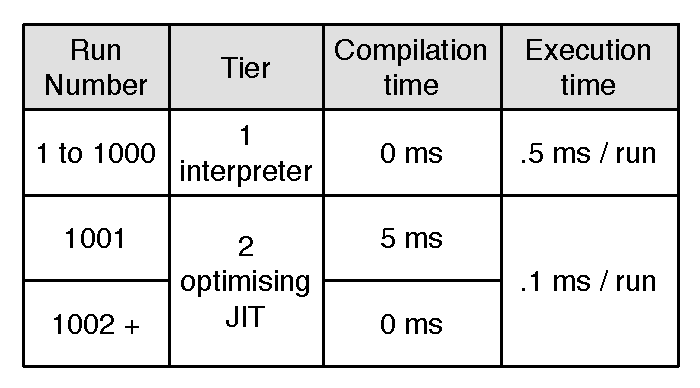
\includegraphics[width=0.5\linewidth]{GeneralTieredArchitecture}
        \caption{Execution of a frequently used code snippet.}
        \label{fig:GeneralTieredArchitecture}
    \end{center}
\end{figure}

\paragraph{Optimising JIT architectures.} Two main architectures are widely used to design an optimising JIT. The first optimising JIT architecture~\cite{UrsPHD}, historically the first one invented, attempts to boost performance by optimising frequently used functions. The native code generated by such optimising JITs are optimised n-functions. We call this architecture the \emph{Function based architecture} and we describe it in Section \ref{sec:architecture}. The second architecture focuses on the optimisation of linear sequences of frequently used instructions. We call this architecture the \emph{Meta-tracing architecture}. Typically, meta-tracing JITs optimise the common execution path of one iteration of each frequently used loop. This second architecture is detailed in Section \ref{sec:metaArchitecture}. As Sista is more similar to the function based architecture, Section \ref{sec:architecture} is more detailed than the other one.

\paragraph{Research problems.} In the context of the design and implementation of the optimising JIT for Pharo, the thesis focuses on 
two
%three 
aspects:
\begin{itemize}
	\item \emph{Metacircular optimising JITs: } Optimising JITs can be written in different programming languages, including the language they optimise. In the latter case, it may be possible for the JIT to optimise its own code. Such aspects are discussed in Section \ref{sec:implLang}.
	\item \emph{Runtime state persistence:} Most modern VMs always start-up an application with only unoptimised code. The application then needs a certain amount of time, called \emph{warm-up time}, to reach peak performance. Warm-up time is a problem if the application needs high-performance immediately. Existing solutions for this problem are detailed in Section \ref{sec:persistence}.
	%\item \emph{Virtual function instruction set:} Most VMs are either only able to execute code from a specific programming language or from a specific virtual function representation. Several modern VMs are able to execute code in other form, for example
\end{itemize}

%what do we discuss
\paragraph{Closed-source VMs.} This chapter tries to discuss the main production and research open-source VMs. Specific closed-source VMs are described as they are relevant in the context the thesis. However, many closed-source VMs are ignored as it is difficult to get reliable and free-to-share information about them, especially if no publications exist on a specific aspect of the VM. 

%Smalltalk.
\paragraph{Smalltalk VMs.} As Pharo is a Smalltalk dialect, it may be interesting to investigate the designs of other Smalltalk VMs. However, commercial Smalltalk VMs in production today are closed-source and do not feature optimising JITs so we do not discuss them. In the 90s, the Self VM~\cite{UrsPHD} and the animorphic VM for Strongtalk~\cite{Sun06} were able to execute Smalltalk code using an optimising JIT. Those VMs are briefly discussed but these VMs are not actively maintained nor used in production.

%%%%%%%%%%%%%%%%%%%%%%%%%%%%%%%%%%%%%%%%%%%%%%%%%%%%%%%%%%%%%%%%%%%%%%%%%%%%%%%%%%%%%%%%%%%%%%%%%%%%%%%%%%%%%%%%%%%%%%%%%%%%%%%%%%%%%%%%%%%%%%%%%%%%%%%%%%%%%%%%%%%%%%%

\section{Terminology}

This section clarifies specific terms to avoid confusion.

\paragraph{Functions.} In the thesis we use the term \emph{function} to refer to executable code, which corresponds in practice to a method or a closure. More specifically, we distinguish \emph{virtual functions}, or v-functions, which can be executed by a virtual machine (in our case, bytecode version of functions) and \emph{native functions}, or n-functions, the native code version of a function executed by a specific processor. 

\paragraph{Frames.} We discuss VMs using an hybrid runtime where v-functions can be executed either through a v-function interpreter or by executing the corresponding n-function generated by a JIT from the v-function. On the one hand, we call \emph{virtual frame} or v-frame a stack frame used by the v-function interpreter. On the other hand, we call \emph{native frame} or n-frame a stack frame used by the execution of a n-function. V-frames have typically a machine-independent representation and all the values used by the execution stored inside the frame, while n-frames may have a machine-dependent representation and may have some values in registers.

\paragraph{Tiered architecture.} One of the most common high-performance VM architecture is the tiered architecture: the first few executions of v-functions are performed by an interpreter and subsequent executions fall into the JIT infrastructure, composed of multiple tiers. Each JIT tier requires more time to compile the v-function to n-function than the previous tier, but the resulting n-function is more efficient. In most VMs, there are two JIT compiler tiers. The first tier is called the \emph{baseline JIT}. It translates quickly v-functions to n-functions with a limited number of optimisations. The baseline JIT typically generates n-functions with inline caches to collect type information. The other tier is called the \emph{optimising JIT}. It translates v-functions to highly optimised n-functions with speculative optimisations, based on the runtime information collected on n-functions generated by the baseline JIT.

\paragraph{Sista.} \emph{Sista} (\textbf{S}peculative \textbf{I}nlining \textbf{S}mall\textbf{T}alk \textbf{A}rchitecture) is the named of the architecture detailed in the thesis. As the architecture has notable differences from the standard tiered architecture, the two runtime compilers are not really a baseline JIT and an optimising JIT. We call them by their project name in the thesis. The first runtime compiler is called \emph{Scorch} and compiles v-functions to optimised v-functions using speculative optimisations. Scorch is written in plain Smalltalk. The second runtime compiler is called \emph{Cogit} and compiles v-functions to n-functions. Cogit can be used alone as the baseline JIT, or as a back-end for Scorch. In the later case, the pair of Scorch and Cogit forms an optimising JIT. Cogit is written in a restrictive Smalltalk compiled ahead-of-time to an executable as part of the VM.

In this context, both v-functions and n-functions can have an optimised version. We therefore used the term v-function to discuss all v-functions (optimised or not), and specify optimised v-function and unoptimised v-function when needed. Similarly, for frames, we say v-frame to discuss v-frames in general, and specify optimised v-frame and unoptimised v-frame when discussing a v-frame respectively representing the execution state of an optimised v-function or a unoptimised v-function. The same terminology is used with native (\emph{n-}) than with virtual (\emph{v-}).

Both runtime compilers can deoptimise stack frames. Cogit can deoptimise any n-frame to a single v-frame. Scorch can deoptimise an optimised v-frame to multiple unoptimised v-frames. 

%%%%%%%%%%%%%%%%%%%%%%%%%%%%%%%%%%%%%%%%%%%%%%%%%%%%%%%%%%%%%%%%%%%%%%%%%%%%%%%%%%%%%%%%%%%%%%%%%%%%%%%%%%%%%%%%%%%%%%%%%%%%%%%%%%%%%%%%%%%%%%%%%%%%%%%%%%%%%%%%%%%%%%%

\section{Function based architecture}
\label{sec:architecture}

The first optimising JIT architecture invented~\cite{UrsPHD} was designed to generate optimised n-functions. From a given v-function, the optimising JIT performs a set of optimisations which includes inlining of other v-functions, and generates an optimised n-function. The section gives firstly an overview of the architecture and then discuss concrete implementations with references in Section \ref{sec:existing1}. The last sections discuss specific aspects of the architecture.

\subsection{Architecture overview}

In most VMs following this architecture, three tiers are present. The following three paragraphs detail each tier, including how virtual calls are executed in each case.

\paragraph{Tier 1: V-function interpreter. } The first tier is a virtual function interpreter. In most VMs, no compilation time is required at all to interpret a v-function\footnote{Some VMs (such as Strongtalk) require compilation time for interpretation because the v-functions are not provided in a format the interpreter can execute (for example source code is provided).} but the execution of the v-function by the interpreter is not very fast. Virtual calls are usually implemented using a global look-up cache to avoid computing the function to activate at each call. The interpreter tier does not necessarily collect runtime information. 
\paragraph{Tier 2: Baseline JIT. } The second tier is the baseline JIT, which generates from a single v-function a n-function with a very limited number of optimisations. Once compiled, the n-function is used to execute the function instead of interpreting the v-function. A small amount of time is wasted to generate the n-function but the execution of the n-function is faster than the v-function interpretation. The n-function generated by the baseline JIT is instrospected to collect runtime information if the function is executed enough times to be optimised by the next tier. The goal of the baseline JIT code generation is therefore to provide reliable runtime information with limited performance overhead over generating efficent n-functions. Virtual calls are usually generated in machine code using inline caches~\cite{Deut84a,Holz91a}: each virtual call has a local cache with the functions it has activated, both speeding-up the execution and collecting runtime information for the next tier.
\paragraph{Tier 3: Optimising JIT. } The last tier is the optimising JIT, which generates an optimised n-function. The optimising JIT uses runtime information such as the inline cache data to speculate on what function is called at each virtual call, allowing to perform inlining and to generate the optimised n-function from multiple v-functions. Such optimisations greatly speed-up execution but are invalid if one of the compile-time speculation is not valid at runtime. In this case, the VM deoptimises the code and re-optimise it differently. The optimising JIT requires more time than the baseline JIT to generate n-functions, but the generated code is much faster. The execution of virtual calls is not really relevant in this tier as most virtual calls are removed through inlining and most of the remaining ones are transformed to direct calls.

\vspace{0.5em}

\begin{figure}[h!]
    \begin{center}
        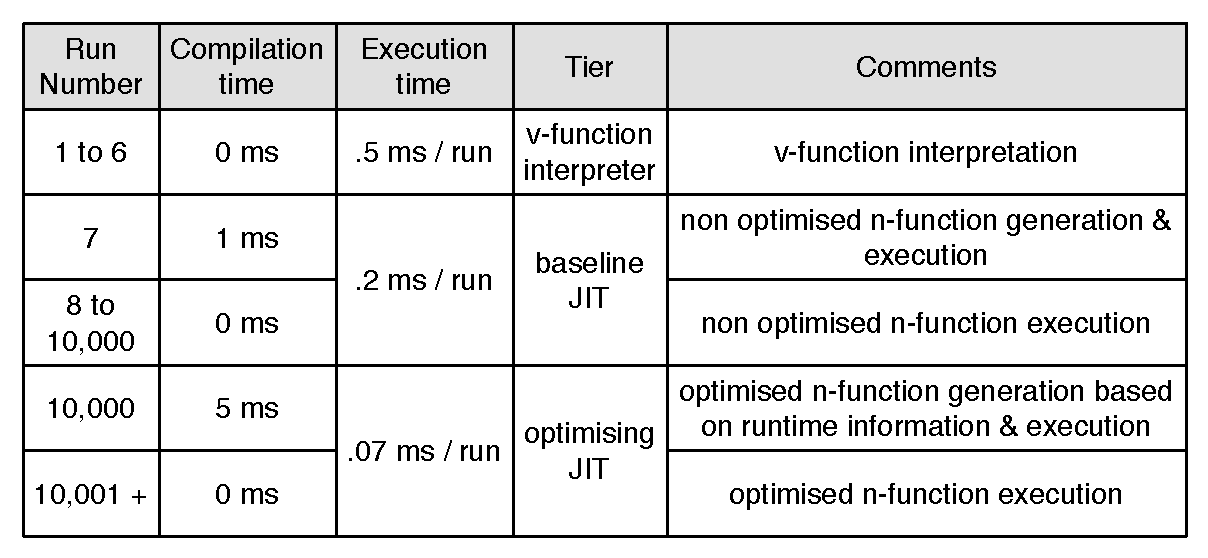
\includegraphics[width=0.95\linewidth]{TieredArchitecture}
        \caption{Execution of a frequently used v-function}
        \label{fig:TieredArchitecture}
    \end{center}
\end{figure}

Figure \ref{fig:TieredArchitecture} shows the theoretical execution of a frequently used v-function over the three tiers. The first few runs are interpreted, each run taking 0.5 ms. The following run requires some compilation time for the baseline JIT to kick in, but the function is then executed 2.5 times faster and runtime information is collected. Lastly, after 10,000 runs, the optimising JIT takes a significant amount of time to generate an optimised n-function. The optimised n-function is executed three times faster than n-function generated by the baseline JIT.

\subsection{Existing virtual machines}
\label{sec:existing1}

The first VM featuring this function based architecture was the Self VM~\cite{UrsPHD}. The Self VM had only two tiers, the baseline JIT and the optimising JIT. The Self programming language has never really become popular so the VM is not really used anymore. 

The second VM built with this design was the Animorphic VM for the Strongtalk programming language~\cite{Sun06}, a Smalltalk dialect. This VM is the first to feature three tiers. The first tier is a threaded code interpreter hence interpretation requires a small amount of compilation time to generate threaded code from the v-function. The two other tiers are the same as in the Self VM. The animorphic VM has never reached production.

The Hotspot VM~\cite{Pale01a} was implemented from the Self and animorphic VM code base and has been the default Java VM provided by Sun then Oracle for more than a decade. In the first versions of the Hotspot VM, two executables were distributed. One was called the client VM, which included only the baseline JIT and was distributed for applications where start-up performance matters. The other one was called the server VM, which included both JIT tiers, and was distributed for application where peak performance matters. Later, the optimising JIT was introduced in the client VM with different optimisation policies than the server version to improve the client VM performance without decreasing too much start-up performance. In Java 6 and onwards, the server VM became the default VM as new strategies allowed the optimising JIT to improve performance with little impact on start-up performance. Lastly, a single binary is now distributed for the 64 bits release, including only the server VM. 

More recently, multiple Javascript VMs were built with a similar design. A good example is the V8 Javascript engine~\cite{V8}, used to execute Javascript in Google Chrome and Node JS. Other VMs, less popular than the Java and Javascript VMs are also using similar architectures, such as the Dart VM. One research project, the Graal compiler~\cite{Oracle13,Dubo13c}, is a function-based optimising JIT for Java that can be used, among multiple use-cases, as an alternative optimising JIT in the Hotspot VM.

\subsection{Just-in-time compiler tiers}

Most VMs featuring this function based architecture have three tiers. The number of tiers may however vary from two to as many as the development team feels like. The following paragraphs discuss the reasons why the VM implementors may choose to implement a VM with two tiers, three tiers or more.

\paragraph{Engineering cost.} Each new tier needs to be maintained and evolved accordingly to the other tiers. Hence, a VM having more tiers requires more engineering time for maintainance and evolutions. Any bug can come from any tier and bugs coming from only a single tier can be difficult to track down. Evolutions need to be implemented on each tier. To lower the VM maintenance and evolution cost, a VM needs to have the least number of tiers possible.

\paragraph{Minimum number of tiers.} By design, the optimising JIT is the key component for high-performance and it needs runtime information from previous runs to generate optimised code. Hence, a VM with the function based architecture requires at least two tiers. One tier, the non-optimising tier, is used for the first runs to collect statistical information and is typically implemented as an interpreter tier or a baseline JIT tier. The second tier, the optimising tier, generates optimised n-functions and is implemented as an optimising JIT. To perform well, the optimising tier has to kick in only if the function is used frequently (else the compilation time would not be worth the execution time saved) and the previous tier(s) must have executed the v-function enough time to have collected reliable runtime information. For this reason, the optimising tier usually kicks in after several thousands executions of the v-function by the previous tier(s).

\paragraph{Two non-optimising tiers.}Most VMs features two non-optimising tiers and one optimising tier. The non-optimising tiers are composed of an interpreter tier and a baseline JIT tier. These two tiers have different pros and cons and featuring both allows the VM to have the best of both worlds. There are three main differences between the two tiers: execution speed, efficiency of runtime information collection and memory footprint. The three differences are detailed in the next three paragraphs.

\subparagraph{Execution speed.} The interpreter tier is faster than the baseline JIT tier if the function is executed a very small number of times because there are not enough executions to outweight the baseline JIT compilation time. Figure \ref{fig:NonOptTierGraph} compares the speed of one to ten executions of the frequently used v-function from Figure \ref{fig:TieredArchitecture}. As interpreting the v-function takes 0.5 ms, the compilation by the baseline JIT 1 ms and the execution of the n-function generated by the baseline JIT 0.2 ms, the interpreter is faster if the v-function is executed less than three times. However, if the function is executed between four times and 10,000 (at which point the optimising JIT kicks in), the baseline JIT tier is faster.

\begin{figure}[h!]
    \begin{center}
        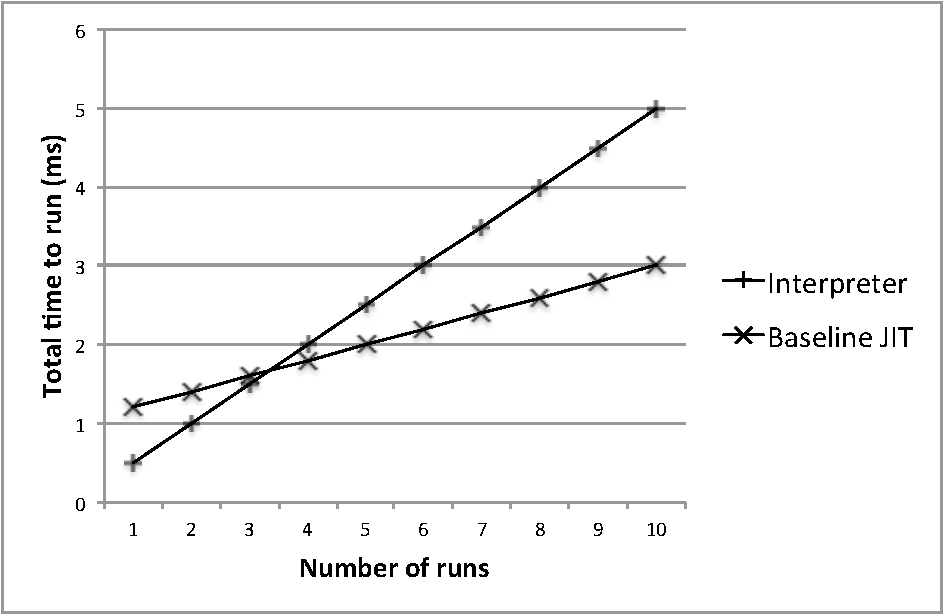
\includegraphics[width=0.70\linewidth]{NonOptTierGraph}
        \caption{Time to execute a v-function in non-optimising tiers}
        \label{fig:NonOptTierGraph}
    \end{center}
\end{figure}
	
	\subparagraph{Runtime information collection.} One of the most relevant runtime information to collect is the function called at each virtual call. It is currently not possible to collect this information without overhead in an interpreter if the interpreter is written in a machine independent language. However, the inline cache technique~\cite{Deut84a,Holz91a} allows one to collect such information in a baseline JIT tier while speeding-up code execution.
	
	\subparagraph{Memory footprint.}The interpreter does not require extra memory for the function it executes as only the v-function representation is needed. On the other hand, the baseline JIT requires memory to store the generated n-function for each v-function it executes. If many functions are executed once, not having the interpreter tier can lead to significant memory overhead.
	
	%\item \emph{Compatibility with optimising JIT: }The code executed by the processor in the interpreter tier is the interpreter code while in the baseline JIT tier is native code. Having both an interpreter and JIT tiers require the runtime to be able to switch efficiently between both runtime, including the management of stack frame representation in both cases.
%\end{enumerate}

\vspace{0.5em}

Having both tiers allows the VM to have a lower memory footprint thanks to the interpreter tier. If the interpreter tier does not collect runtime information and is used only for the first few executions, the start-up performance is much better when both tiers are present than when one or the other is present alone. Runtime information can be collected with little overhead thanks to the baseline JIT tier. For these reasons, many VMs feature these two non-optimising tiers. 

A good example of the pros and cons of multiple tiers is the evolution of the V8 Javascript engine~\cite{V8}. In 2008, the first version was released featuring only the baseline JIT tier. The following year, the optimising JIT tier was added to improve performance. In 2016, the interpreter tier was added both to lower the memory footprint and to improve start-up performance.

In general, the two non-optimising tiers are kept as simple as possible to ease maintainance and evolutions. Only the third tier, the optimising JIT, may be more complex to be able to generate efficient n-functions.

\paragraph{More than three tiers.} Adding more than three tiers is usually not worth it as it would mean additional maintenance and evolution cost. However, in specific languages such as Javascript where the start-up performance is critical, it can be worth it to have two optimising JIT tiers to increase start-up performance. The Javascript Webkit VM has four tiers since 2015~\cite{Webkit15}. In this case, the VM team introduced two optimising JIT tiers after the interpreter and baseline JIT. One optimising JIT tier has smaller compilation time than the other one but produce less efficient n-function.

\paragraph{Independant compiler tiers.}
In most VMs, the baseline JIT and the optimising JIT are completely independant entities. Indeed, both JIT tiers are fundamentally different and it is difficult to share code between both tiers. 

\subparagraph{Baseline JIT.} The baseline JIT has to be as simple as possible to limit the maintenance cost, simplicity is more important than generated code quality as most of the VM performance comes from the optimising JIT. The n-function it generates needs to be easily introspected to collect runtime information about the previous runs for the optimising JIT to direct compiler optimisations. The baseline JIT compilation time has to be very small.

The baseline JIT is typically implemented as a template-based engine~\cite{Deut84a}, generating a predefined sequence of native instructions for each virtual instruction. Template-based generation engines are relatively simple to implement and maintain. Templates are very convenient for native code introspection because the JIT knows the exact sequence of native instructions generated for each virtual instruction so it knows the exact bytes to read to extract runtime information. Lastly, template-based compilation is usually very efficient, providing low compilation time.

\subparagraph{Optimising JIT.} The optimising JIT is significantly different. It needs to generate n-functions as efficient as possible with a reasonnable compilation time, but potentially much higher than the baseline JIT. The n-functions generated by the optimising JIT are in most VMs not introspected, allowing the optimising JIT to generate the most efficient instructions. As any software project, complexity has to be controlled but it is usually worth to add complexity in the optimising JIT to allow it to generate more efficient code as it leads to overall better VM performance. The optimising JIT is typically implemented, as shown in Figure \ref{fig:OptJITFig}, by translating the v-function to a high-level intermediate representation to perform language-specific optimisations. It then transforms the representation to another intermediate representation, closer to native instruction, where machine-specific optimisations are performed. Lastly it generates native code.

\begin{figure}[h!]
    \begin{center}
        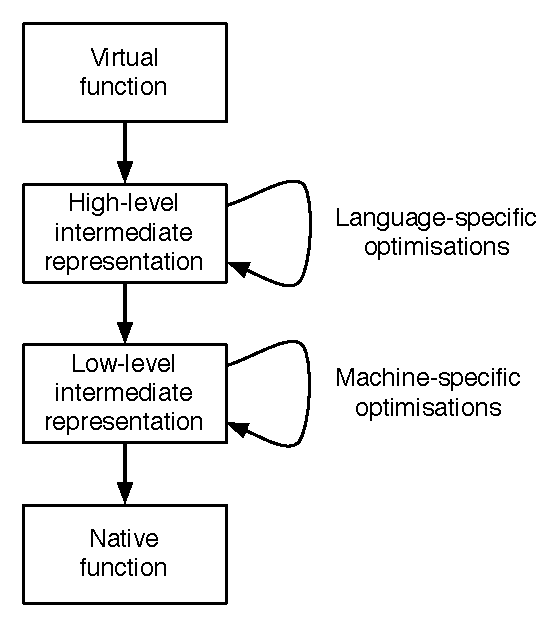
\includegraphics[width=0.49\linewidth]{OptJITFig}
        \caption{Classical optimising JIT architecture}
        \label{fig:OptJITFig}
    \end{center}
\end{figure}

\paragraph{Sharing code between compiler tiers.} Because of the fundamental differences, most optimising JITs use a completely different code base than the baseline JIT they work with. However, there are some rare cases where part of the JIT compilers are shared between multiple tiers. 

The first case is the Javascript Webkit VM~\cite{Webkit15}. As four tiers are present, it is possible to share portions of the compilers because some features are required in multiple tiers. For example, both the baseline JIT and the first-level optimising JIT requires the VM to be able to instrospect the generated machine code. In addition, both optimising JITs have optimisation logic in common allowing to share part of the optimisation pipeline. In this case, they share the high-level optimisations while the low-level optimisations are done in different back-ends.

The second case is related to VM extensions. The Javascript VMs are now attempting to support, in addition of Javascript, an abstract assembly language called WebAssembly~\cite{WebAssembly}. WebAssembly allows the programmer to compile ahead-of-time specific frameworks or libraries for use-cases difficult to optimise efficiently at runtime, such as real-time libraries. WebAssembly provides both abstract assembly code instructions and convenient instructions to interface WebAssembly with Javascript and the web page. In the V8 Javascript engine~\cite{V8}, the low-level intermediate representation of TurboFan, the optimising JIT of V8, is shared between the WebAssembly back-end and the optimisation path for Javascript code.

\subsection{Concurrent compilation}

The first optimising JIT, designed and implemented in Self~\cite{UrsPHD}, was done in single-threaded environment. In this case, the optimising JIT had a limited time period to produce optimised code, and if the time period was not enough, the function was not optimised. Since the early 2000s, multi-threaded environments have become more common and many optimising JITs now perform optimisations concurrently to the application native thread(s)~\cite{Arn00,Stad12a}.

In most cases, not all the runtime compilations are however done concurrently. The baseline JIT is typically executed in the same native thread than the application. As it has very small compilation time, the compilation time overhead is usually not significant enough to justify concurrent compilation. When a frequently used portion of code is detected, the optimising JIT has to choose a function to optimise based on the current stack. This cannot be done concurrently as the stack needs to be introspected. Once the function to optimise is chosen, the optimisation of the function can be done concurrently. The optimising JIT has usually access to a pool of native threads which take functions to optimise in a compilation queue, optimises them and installs them. Further calls on such functions can use the optimised version installed. However, the optimising JIT may insert guards to ensure assumptions speculated at compile-time (such as the type of a specific variable) are valid at runtime. If one of the guard fails, the stack needs to be deoptimised to resume with non-optimised code. Deoptimisation of the stack is not done concurrently as the application requires the deoptimisation to be finished to resume execution. 

\subsection{Aosta technical report}

Normally technical reports are not relevant enough to be mentioned, but as Sista is based on the Aosta technical report\cite{Mira02c}, it is definitely worth talking about it.

Aosta is a design sketch for an adaptive optimiser implemented in Smalltalk above a conventional Smalltalk virtual machine (a virtual machine featuring a baseline JIT) with \emph{minor} extensions. Adaptive optimisation are discussed in the sense of Urs H\"olzle \cite{UrsPHD}. The sketch is far from complete, focusing instead on the interface between the optimiser and the virtual machine, hence outlining a potentially portable architecture where an optimiser written in Smalltalk can be hosted above a range of specific virtual machines. This portability is intended to allow the Smalltalk community to collaborate on the project without having to define and implement a common VM, with all the difficulties of migrating current systems to a new VM, allowing the community to apply the optimiser within the existing systems.  Of course, this architecture still requires significant extensions to the execution machinery of existant VMs but these extensions amount to something far from a rewrite.

The sketch is then detailed in the context of HPS, the VisualWorks VM, which is a second generation implementation of Peter Deutsch's PS Smalltalk~\cite{Deut84a}. The author chose to describe the architecture with this VM as he is familiar with it and the sketch needed (according to the author) to be based on an existing VM to make it as real as possible. The sketch is expected to apply more broadly than just HPS but this is yet to prove. The sketch was, in 2002, functioning as a specification for the HPS implementation. 

%%%%%%%%%%%%%%%%%%%%%%%%%%%%%%%%%%%%%%%%%%%%%%%%%%%%%%%%%%%%%%%%%%%%%%%%%%%%%%%%%%%%%%%%%%%%%%%%%%%%%%%%%%%%%%%%%%%%%%%%%%%%%%%%%%%%%%%%%%%%%%%%%%%%%%%%%%%%%%%%%%%%%%%

\section{Meta-tracing architecture}
\label{sec:metaArchitecture}

The main alternative to the function based architecture is the meta-tracing architecture. Meta-tracing JITs do not optimise entire functions but instead focus on optimising linear sequences of instructions. As most meta-tracing JITs focus on the optimisation of loop iterations, we detail this case in this section. The section starts by providing an overview of the architecture and then discusses concrete implementation with references in Section \ref{sec:existing2}.

\subsection{Architecture overview}

VMs with meta-tracing JITs generate optimised native code only for the frequently used paths of commonly executed loops and interpret virtual instructions for the rest of the program. Tracing JITs are built on the following basic assumptions:
\begin{itemize}
	\item Programs spend most of their runtime in loops.
	\item Several iterations of the same loop are likely to take similar code paths.
\end{itemize}

Typically, in VMs with tracing JITs, the first executions of a loop are done using a v-function interpreter. The interpreter profiles the code executed to detect frequently used loop, usually by having a counter on each backward jump instruction that counts how often this particular backward jump is executed. When a hot loop is identified, the interpreter enters a special mode, called tracing mode. During tracing, the interpreter records a history of all the operations it executes during a single execution of the hot loop. The history recorded by the tracer is called a trace: it is a list of operations, together with their actual operands and results. Such a trace can be used to generate efficient native code. This generated machine code is immediately executable and can be used in the next iteration of the loop.

Being sequential, the trace represents only one of the many possible paths through the code. To ensure correctness, the trace contains a guard at every possible point where the path could have followed another direction, for example at conditional branches or virtual calls. When generating native code, every guard is turned into a quick check to guarantee that the path we are executing is still valid. If a guard fails, the execution immediately quits the native code and resumes the execution by falling back to the interpreter.

\subsection{Existing VMs}
\label{sec:existing2}

Tracing optimisations were initially explored by the Dynamo project~\cite{Bala00a} to dynamically optimise native code at runtime. Its techniques were then successfully used to implement a JIT compiler for a Java VM~\cite{Gal06a}. The technique was used in Mozilla's JavaScript VM from Firefox 3 to Firefox 11~\cite{Gal09a} until Mozilla removed it to replace it by a function-based JIT. 

The most famous meta-tracing JITs in production are certainly the ones generated from the RPython toolchain~\cite{Rigo06a}. The RPython toolchain allows the generation of a meta-tracing JIT for free if one writes a virtual function interpreter in RPython. The most popular example is Pypy~\cite{Rigo06a,PyPyTracing}, a Python VM using a meta-tracing JIT through the RPython toolchain framework.

\subsection{Sista and metatracing JITs}

Sista was not designed as a metatracing JIT. There were two main reasons. First, the design was inspired from the Aosta proposal, which is a function-based architecture design. Second, we did not believe that optimising loop bodies would make sense in the context of Smalltalk and we explain why in the second paragraph of Section \ref{sec:relWArch}.

%%%%%%%%%%%%%%%%%%%%%%%%%%%%%%%%%%%%%%%%%%%%%%%%%%%%%%%%%%%%%%%%%%%%%%%%%%%%%%%%%%%%%%%%%%%%%%%%%%%%%%%%%%%%%%%%%%%%%%%%%%%%%%%%%%%%%%%%%%%%%%%%%%%%%%%%%%%%%%%%%%%%%%%

\section{Metacircular optimising Just-in-time compiler}
\label{sec:implLang}

An optimising JIT is implemented in a programming language and is able to optimise code from one or multiple programming languages. If the implementing language of the optimising JIT is one of the language it can optimise, is the optimising JIT able to optimise its own code ?

The section starts by discussing the programming languages in which the optimising JITs are written. For the rare case where the implementing language of an optimising JIT is included in the languages the JIT can optimise, we detail if such optimisations are possible and used in production.

\subsection{Implementation language}
Historically, VMs have been implemented in low-level languages such as C++. Low-level languages are very convenient for multiple VM development tasks, such as direct memory access or optimisation of specific portion of the VM code for performance. The first optimising JITs, including the Self, Animorphic and Java Hotspot VMs~\cite{UrsPHD,Sun06} were written in C++. More recently, Javascript VMs such as V8 or Webkit~\cite{Webkit15} were still written in C++. As far as we know, there is no optimising JIT in production optimising C++ code, hence none of these JITs are able to optimise their own code.

Another approach is to use a high-level language compiled ahead-of-time to assembly code to write the optimising JIT. This approach is used by the RPython toolchain~\cite{Rigo06a}, where RPython is a restricted Python that can be compiled to native code through C. RPython was used to write Pypy's meta-tracing optimising JIT. In the case of Pypy, the JIT is able to optimise Python code, and as RPython is a subset of Python, the JIT is able to optimise its own code. However, in production, all the RPython code is compiled ahead-of-time to an executable binary. All the JIT code base is therefore translated to native code, and as the JIT cannot optimise native code, the JIT does not optimise itself in production.

Figure \ref{fig:RPythonVMCompilation} shows the compilation of the production VM using RPython. The Core VM is written in RPython, and the RPython to C compiler generates C files from the RPython code. The final VM is compiled using a C compiler from the generated C files and additional C files for platform-specific code.

\begin{figure}[h!]
    \begin{center}
        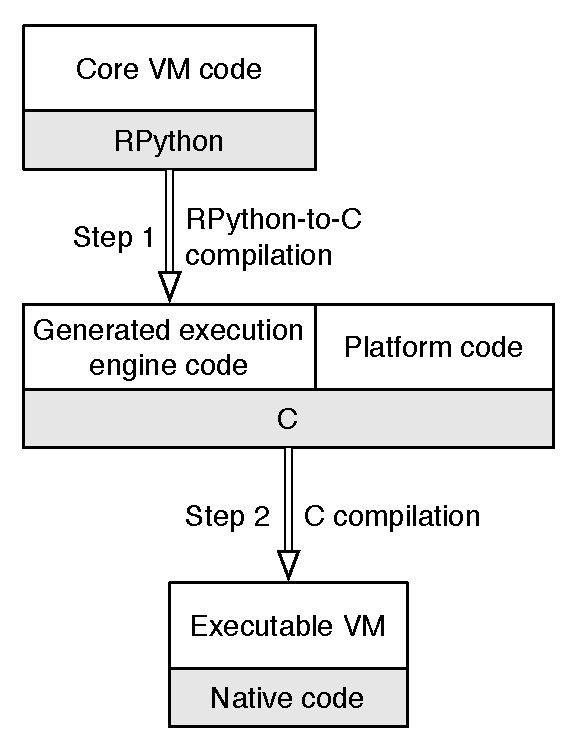
\includegraphics[width=0.45\linewidth]{RPythonVMCompilation}
        \caption{RPython VM executable generation}
        \label{fig:RPythonVMCompilation}
    \end{center}
\end{figure}

\paragraph{Metacircular VMs.} Multiple research projects showed that it is possible to implement an entire VM in the programming language the VM runs. Such VMs are called metacircular VMs. 

The Jalape\~no project, now called Jikes RVM~\cite{Alp99a}, was the first successful VM with such a design. Jikes RVM is a Java VM written in Java. On the Jikes RVM official page, it is written that the current version of the VM does not perform runtime optimisations based on runtime information. There is however a runtime compiler present in Jikes RVM~\cite{Arn00} optimising the code more aggressively than the baseline JIT, but it does not seem to use runtime information to direct its optimisations. 

%TODO Disambig metacircular VM.

Another Java VM written in Java was implemented in the late 2000s at Oracle, called Maxine VM~\cite{Wimm13a}. Maxine had multiple working optimising JITs. The most popular was extracted from the Maxine VM and is now known as the Graal compiler~\cite{Oracle13,Dubo13c}. In the case of Maxine, the optimising JIT is written in Java and is able to optimise its own code.

There were other attempts to implement meta-circular VMs for other languages than Java. The Klein VM~\cite{Unga05b} is a Self VM written in Self and reportedly, in 2009, there was some work in the direction of an optimising JIT. The project does not seem however to be very active today and the optimising JIT is definitely not fully working. There is even an attempt to write a Smalltalk VM in Smalltalk~\cite{Pim14a}, called Bee Smalltalk. Unfortunately, as of today, Bee Smalltalk is not open-source and it is not clear if an optimising JIT is present or not.

The last but not least project is the Truffle framework~\cite{Wur13a}. Truffle is a framework allowing to write efficiently VMs for different programming languages. The Truffle runtime is built on top of Java's Hotspot VM, but the Graal compiler is used as the optimising JIT instead of the Hotspot optimising compiler. 
Multiple VMs using the Truffle framework were implemented for different programming language in the past years. For each of them, the Graal compiler in the Truffle runtime can optimise both Java code and the programming language run. As Graal is written in Java, it can optimise its own code.
 
\subsection{Optimising Just-in-time compiler optimising itself}

Overall, very few optimising JITs are written in a programming language they can optimise. Even when they could optimise themselves, the VM development team may choose to compile the JIT code to native code ahead-of-time and the optimising JIT does not optimise itself in production. The main existing case where the optimising JIT is optimising its own code is the Graal optimising JIT. Graal can be used in different contexts. It was built as the Maxine VM optimising JIT. It is now mainly used as the optimising JIT of the Truffle runtime, as an alternative optimising JIT for Java Hotspot.

We detail here briefly how the Graal compiler optimise its own code when it is running as an alternative optimising JIT in the Java Hotspot VM. In this case, the Graal optimising JIT is written in Java while the rest of the VM, originally from the Java Hotspot VM, are written in C++. The application is running using multiple native threads and the Graal compiler is running in other native threads, concurrently.

When a frequently used portion of code is detected, the Hotspot VM chooses a function to optimise based on the current stack. The VM then puts the function to optimise in a thread-safe compilation queue. The Graal compiler native threads, running concurrently to the application, take functions to optimise in the compilation queue and generate an optimised function for function in the queue. Hotspot provides APIs to extract runtime information from each unoptimised function to direct the compiler optimisation. Once the optimisation finished, the Graal compiler provides to Hotspot an optimised n-function with deoptimisation metadata. The Hotspot VM may install the optimised n-function. If one of the compilation-time assumption is invalid at runtime, the Hotspot VM is able to deoptimise the stack based on the deoptimisation metadata provided by the Graal compiler.

%%%%%%%%%%%%%%%%%%%%%%%%%%%%%%%%%%%%%%%%%%%%%%%%%%%%%%%%%%%%%%%%%%%%%%%%%%%%%%%%%%%%%%%%%%%%%%%%%%%%%%%%%%%%%%%%%%%%%%%%%%%%%%%%%%%%%%%%%%%%%%%%%%%%%%%%%%%%%%%%%%%%%%%

\section{Runtime state persistence}
\label{sec:persistence}

In Sista, we persist the runtime state across multiple start-ups, including the optimised code but also the running green threads using optimised code. Persistence of running green thread with optimised code has not been done before. In our case, we need to persist green threads as the normal Smalltalk developer workflow requires it. It seems no other programming language with an optimising JIT have the same requirement so the running green threads are not persisted across start-ups. For this reason, we focus in this section on the persistence of optimised code between multiple start-ups.

One of the main problems with optimising JITs, compared to ahead-of-time compiler, is the start-up performance. As the optimising JIT needs runtime information to optimise code, usually thousands of unoptimised runs of a code snippet are required before reaching peak performance. This warm-up time can cause significant problems in specific short-lived applications, where most of the execution time is spent before reaching peal performance. 
%In addition, the warm-up time implies additional energy consumption (the processor needs to optimise code, consuming energy) at each application start-up, which is a problem in specific use-cases such as mobiles where battery consumption is critical.

Because of these constraints, some object-oriented languages are compiled with an ahead-of-time compiler. Static analysis is performed over the code to guess what function is called at each virtual call. Applications for the iPhone are a good example where static analysis is used to pre-optimise the Objective-C application. The peak performance is lower than with a JIT compiler if the program uses a lot of virtual calls, as static analysis is not as precised as runtime information on highly dynamic language. However, if the program uses few dynamic features (for example most of the calls are not virtual) and is running on top of a high-performance language kernel like the Objective-C kernel, the result can be satisfying.

Most object-languages still choose to run on top of a VM with an optimising JIT. The section describes four existing techniques to improve start-up performance, including techniques related to optimised code persistence across start-ups.

\paragraph{Many tiers architecture.}
One solution to decrease warm-up time is to have many tiers in the function based architecture. The idea is that code would be executed slowly the few first iterations, a bit faster the next iterations, faster after an certain number of optimisations, and so on. Instead of being slow for many iterations before being fast, the VM can this way have a very good trade off between compilation time, runtime information quality and code performance.

The best example is the Javascript Webkit VM~\cite{Webkit15}. A code snippet is:
\begin{enumerate}
\item Interpreted by a bytecode interpreter the first 6 executions.
\item Compiled to machine code at 7th execution, with a non-optimising compiler, and executed as machine code up to 66 executions.
\item Recompiled to more optimised machine code at 67th execution, with an optimizing compiler doing some but not all optimisations, up to 666 executions.
\item Recompiled to heavily optimised machine code at 667th execution, with all the optimisations.
\end{enumerate}

At each step, the compilation time is greater but the execution time decreases. The many tiers approach (four tiers in the case of Webkit), allows the VM to have decent performance during start-up, while reaching high performance for long running code. However, this technique has a severe drawback: the VM team needs to maintain and evolve many different tiers.

\paragraph{Persisting runtime information.}

To reach quickly peak performance, one way is to save the runtime information, especially inlining decisions made by the optimising JIT. In 
 \cite{Sun06}, it is possible to save the inlining decision of the optimising compiler in a separate file. The optimising compiler can then reuse this file to take the right inlining decision in subsequent start-ups. In \cite{Arno05c}, the profiling information of unoptimised runs is persisted in a repository shared by multiple VMs, so new runs of the VM can re-use the information to direct compiler optimisations.

\paragraph{Persisting machine code.}

In the Azul VM Zing~\cite{Azul}, available for Java, the official web site claims that "operations teams can save accumulated optimizations from one day or set of market conditions for later reuse" thanks to the technology called \emph{Ready Now!}. In addition, the website precises that the Azul VM provides an API for the developer to help the JIT to make the right optimisation decisions. 

As Azul is closed source, implementation details are not entirely known. However, word has been that the Azul VM reduces the warm-up time by saving machine code across multiple start-ups. If the application is started on another processor, then the saved machine code is simply discarded. It is very difficult to persist optimised native code across multiple start-ups due to position dependent code and low-level details, but with the example of Azul, we know it is possible.

Aside from Azul, the work of Reddi and all~\cite{Redd07a} details how they persist the machine code generated by the optimising JIT across multiple start-ups of the VM. JRockit~\cite{JRockit}, an Oracle product, is a production Java VM allowing to persist the machine code generated by the optimising JIT across multiple start-ups.

\paragraph{Preheating through snapshots}

\paragraph{Dart snapshots.}
The Dart programming language features snapshots for fast application start-up. In Dart, the programmer can generate different kind of snapshots \cite{Anna13a}. The Dart team added in 2016 two new kind of snapshots, specialized for iOS and Android application deployment.

\subparagraph{Android.} A Dart snapshot for an Android application is a complete representation of the application code and the heap once the application code has been loaded but before the execution of the application. The Android snapshots are taken after a warm-up phase to be able to record call site caches in the snapshot. The call site cache is a regular heap object accessed from machine code, and its presence in the snapshot allows one to persist type feedback and call site frequency.

\subparagraph{iOS.} For iOS, the Dart snapshot is slightly different as iOS does not allow JIT compilers. All reachable functions from the iOS application are compiled ahead of time, using only the features of the Dart optimising compiler that don't require dynamic deoptimisation. A shared library is generated, including all the instructions, and a snapshot that includes all the classes, functions, literal pools, call site caches, etc.

\paragraph{Cloneable VMs.}
In Java, snapshots are not available and used by default. However, Kawachiya and all describe in their work~\cite{Kawa07a} extensions to a Java VM to be able to clone the state of a running Java VM in a similar way to snapshots. In this work, the cloned VM duplicates the heap but also the machine code generated by the different JIT tiers.

%%%%%%%%%%%%%%%%%%%%%%%%%%%%%%%%%%%%%%%%%%%%%%%%%%%%%%%%%%%%%%%%%%%%%%%%%%%%%%%%%%%%%%%%%%%%%%%%%%%%%%%%%%%%%%%%%%%%%%%%%%%%%%%%%%%%%%%%%%%%%%%%%%%%%%%%%%%%%%%%%%%%%%%

%\section{Virtual machine interface}

%\subsection{The Graal-Hotspot architecture}

%+ Graal and interface

%\subsection{WebAssembly}

%WebAssembly 

%%%%%%%%%%%%%%%%%%%%%%%%%%%%%%%%%%%%%%%%%%%%%%%%%%%%%%%%%%%%%%%%%%%%%%%%%%%%%%%%%%%%%%%%%%%%%%%%%%%%%%%%%%%%%%%%%%%%%%%%%%%%%%%%%%%%%%%%%%%%%%%%%%%%%%%%%%%%%%%%%%%%%%%

\section*{Conclusion} 

This chapter detailed existing solutions for our research problems, including the existing optimising JIT architectures, their implementation languages and how some VMs persist optimised code across multiple start-ups. The following chapter describes the existing Pharo runtime which was used as a starting point for our implementation.

%%%%%%%%%%%%%%%%%%%%%%%%%%%%%%%%%%%%%%%%%%%%%%%%%%%%%%%%%%%%%%%%%%%%%%%%%%%%%%%%%%%%%%%%%%%%%%%%%%%%%%%%%%%%%%%%%%%%%%%%%%%%%%%%%%%%%%%%%%%%%%%%%%%%%%%%%%%%%%%%%%%%%%%

%FOLLOWING IS OLD VERSION FOR HISTORY.

%In this chapter, the most popular production VMs and relevant research VMs are discussed. In further chapter, the thesis' proposed architecture will be compared against those VMs. 

%Most popular production VMs, such as Java Hotspot (Cite) or Javascript's V8 (Cite) VMs are written in C++. Using C++ as a performance oriented low-level programming language proved to be very effective as it is possible to write code in a performance oriented fashion. A clear separation is made between the VM and the programming language run so there are no metacircular problems.

%Most of those VMs start-up from the language kernel, a set of core librairies and either source files or files containing bytecodes. Reaching peak performance takes a certain amount of time as the VM needs to detect and optimise correctly frequently used patterns of code. Reportedly, this warm-up time can be from several milliseconds up to multiple days. To solve partially the warm-up problem, such VMs are built with a tiered-architecture: the first few executions are run slowly but without any compilation time, subsequent hundreds of executing are run a bit faster with limited compilation time while further execution are run at peak performance after a certain amount of compilation time.

%An interesting point ot note is that several mainstream VMs were led by the same person (Lars Bak), who became very good at implementing very efficient and easy-to-maintain VMs in C++ as he implemented multiple of those in his life. His work therefore pushed the direction of VM implementation in the C++ direction.

%Among the C++ virtual machines, we will detail two specific VMs have uncommon features that are relevant in the context of the thesis. 

%\subsection{Azul}
%The Azul VM \cite{Azul} is a closed-source VM and expensive VM for Java. As for all closed-source projects, no one external to the project can be certain of what the code is doing. However, word has been that the Azul VM is able to persist optimised machine code across multiple start-ups. If the application is started on another processor, then the saved machine code is simply discarded. 

%\subsection{Dart}
%The Dart VM is an open-source VM for the Dart programming language. Dart features snapshots for fast application start-up. In Dart, the programmer can generate different kind of snapshots \cite{Anna13a}. Since that publication, the Dart team have added two new kind of snapshots, specialized for iOS and Android application deployment, which are quite similar to our snapshots.


%As the sista architecture is implemented in the context of Smalltalk, it could be relevant to discuss existing Smalltalk virtual machines. These VMs are interesting for multiple reasons, but unfortunately many of the Smalltalk virtual machines in production today are closed-source, making the discussion around them not that relevant as information is missing and unaccessible. In addition, as far as we know, there are no production Smalltalk VM today with an optimising JIT compiler, so the comparison with such VMs is even less relevant. 

%However, speculative optimisations in VMs started with the Self VM (CITE), with Self being a Smalltalk-like language, and was followed up with the strongtalk VM (CITE). Both VMs are open-source and available today but none of them are used in production. Self had never really broken through mainstream programming while strongtalk had never reached production state.

\ifx\wholebook\relax\else
    \end{document}
\fi